\documentclass[11pt]{article}

\usepackage{amsmath}
\usepackage{amssymb}

\usepackage{graphicx}
\usepackage{tikz}

\usepackage{ytableau}

\title{Matchings, \\UMTYMP Advanced Topics, Fall 2020}
\author{}
\date{}

\begin{document}

\maketitle

\begin{enumerate}
\item Let $G$ be the following bipartite graph on 12 vertices:
\[\includegraphics[width=1in]{matching.png}\]
Find a matching of $G$ with the maximum possible number of edges. How do you \emph{know} that this is the maximum?

\item Let $G$ be a bipartite simple graph with bipartition $(X,Y)$. Suppose that $n=|X|=|Y|$ (so the total number of vertices of $G$ is $2n$).
\begin{enumerate}
\item Suppose $G$ has a perfect matching. Must it be connected?
\item What is the fewest number of edges $G$ could have if it has a perfect matching.
\item Show that $G$ can have $n^2-n$ edges but still fail to have a perfect matching.
\item Can $G$ have $n^2-n+1$ edges and fail to have a perfect matching? Explain why not, or give an example. (This question is a bit {\bf tricky}.) 
\end{enumerate}

\pagebreak

\item How many perfect matchings does the complete bipartite graph $K_{n,n}$ have?

\item Let $G$ be the $2\times n$ \emph{grid graph}:
\[ 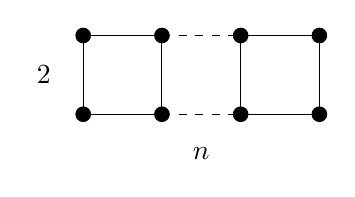
\begin{tikzpicture}
\node at (-0.5,0.5) {$2$};
\node[fill=black, circle, inner sep=2pt] at (0,0) {};
\node[fill=black, circle, inner sep=2pt] at (0,1) {};
\node[fill=black, circle, inner sep=2pt] at (1,0) {};
\node[fill=black, circle, inner sep=2pt] at (1,1) {};
\node[fill=black, circle, inner sep=2pt] at (2,0) {};
\node[fill=black, circle, inner sep=2pt] at (2,1) {};
\node[fill=black, circle, inner sep=2pt] at (3,0) {};
\node[fill=black, circle, inner sep=2pt] at (3,1) {};
\draw (0,0) -- (0,1) -- (1,1) -- (1,0) -- (0,0);
\draw[dashed] (1,0) -- (2,0);
\draw[dashed] (1,1) -- (2,1);
\draw (2,0) -- (2,1) -- (3,1) -- (3,0) -- (2,0);
\node at (1.5,-0.5) {$n$};
\end{tikzpicture} \]
\begin{enumerate}
\item Show that $G$ is bipartite (describe the bipartition $(X,Y)$).
\item Compute the number of perfect matchings of $G$ for $n=1,2,3,4$.
\item Do you recognize this sequence of numbers (we've seen it before!)? Can you prove why, for general $n$, it is the sequence we've seen before?
\end{enumerate}
\end{enumerate}

\noindent {\bf Remark}: Kasteleyn showed that the number of the number of matchings of the more general $m \times n$ grid graph is:
\[ \left(\prod_{j=1}^{m} \prod_{k=1}^{n} \left( 4 \cos^2\left( \frac{\pi j}{m+1} \right) + 4\cos^2 \left( \frac{\pi k}{n+1} \right)\right) \right)^{1/4}.\]
What a crazy formula, huh?! Behind this formula are some \emph{linear algebra} techniques, like the computation of a certain \emph{determinant}. This is kind of similar to, but more advanced than, the Matrix-Tree Theorem we saw for computing the number of spanning trees as a determinant.

\end{document}
